\section{Short introduction to parallel Haskells}
There are already several ways to write parallel programs in Haskell. As we will base our parallel arrows on existing parallel Haskells, we will now give a short introduction to the ones we use as backends in this paper.

In its purest form, parallel computation (on functions) can be looked at as the execution of some functions \code{a -> b} in parallel:

\begin{lstlisting}[frame=htrbl]
parEvalN :: [a -> b] -> [a] -> [b]
\end{lstlisting}
\begin{center}
	\includegraphics[scale=0.7]{images/parEvalN}
\end{center}
We will now implement \code{parEvalN} with the different parallel Haskells.

\subsection{Multicore Haskell}
Multicore Haskell \cite{multicore_hackage} is the GHC native way to do parallel processing. It ships with parallel evaluation strategies for several types which can be applied with \code{using :: a -> Strategy a -> a}. For \code{parEvalN} this means that we can just apply the list of functions \code{[a -> b]} to the list of inputs \code{[a]} by zipping them with the application operator \code{\$}. This lazy list \code{[b]} is then forcibly evaluated in parallel with the strategy \code{Strategy [b]} by the \code{using} operator. This strategy can be constructed with \code{parList :: Strategy a -> Strategy [a]} and \code{rdeepseq :: NFData a => Strategy a}.

\begin{lstlisting}[frame=htrbl]
parEvalN :: (NFData b) => [a -> b] -> [a] -> [b]
parEvalN fs as = zipWith ($) fs as `using` parList rdeepseq
\end{lstlisting}
\begin{center}
	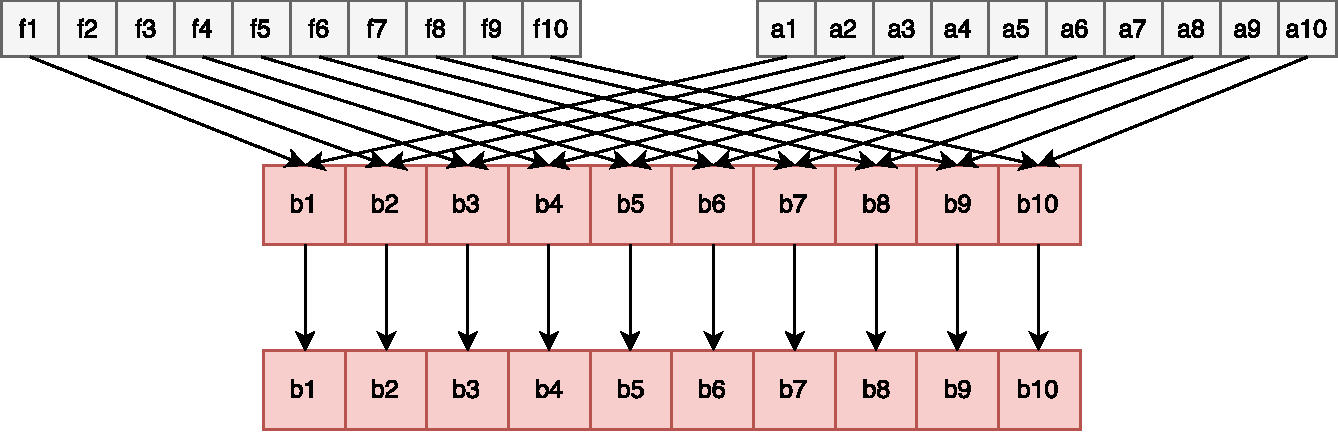
\includegraphics[scale=0.5]{images/parEvalNMulticore}
\end{center}

\subsection{ParMonad}
The \code{Par} monad introduced by Marlow et al. \cite{monad_par_paper_2011}, which can be found in the monad-par package on hackage \cite{monad_par_hackage}, is a monad designed for composition of parallel programs.
\\\\
Our parallel evaluation function \code{parEvalN} can be defined by zipping the list of \code{[a -> b]} with the list of inputs \code{[a]} with the application operator \code{\$} just like with Multicore Haskell. Then, we map over this not yet evaluated lazy list of results \code{[b]} with \code{spawnP :: NFData a => a -> Par (IVar a)} to transform them to a list of not yet evaluated forked away computations \code{[Par (IVar b)]}, which we convert to \code{Par [IVar b]} with \code{sequenceA}. We wait for the computations to finish by mapping over the \code{IVar b}'s inside the \code{Par} monad with \code{get}. This results in \code{Par [b]}. We finally execute this process with \code{runPar} to finally get \code{[b]} again.

\begin{lstlisting}[frame=htrbl]
parEvalN :: (NFData b) => [a -> b] -> [a] -> [b]
parEvalN fs as = runPar $ 
	(sequenceA $ map (spawnP) $ zipWith ($) fs as) >>= mapM get
\end{lstlisting}
\begin{center}
	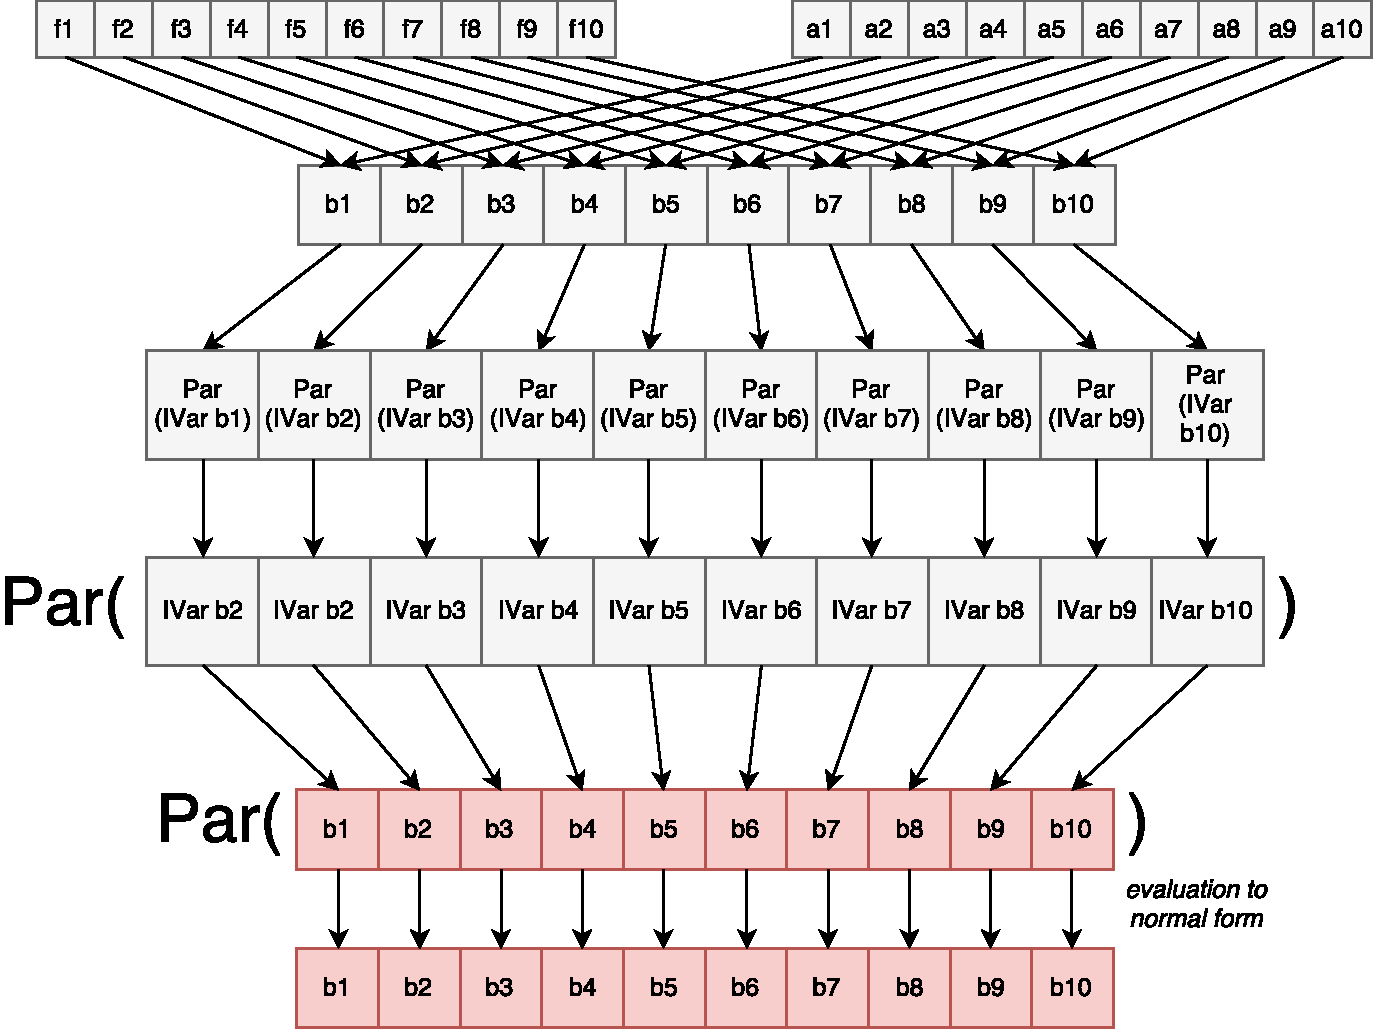
\includegraphics[scale=0.5]{images/parEvalNParMonad}
\end{center}

\subsection{Eden}
Eden  is a parallel Haskell for distributed memory and comes with a MPI and a PVM backend \cite{eden_hackage, Loogen2012, eden_homepage}. This means that it works on clusters as well so it makes sense to have a Eden-based backend for our new parallel Haskell.
\\\\
While it also comes with a monad \code{PA} for parallel evaluation, it also ships with a completely functional interface that includes
\\
\code{spawnF :: (Trans a, Trans b) => [a -> b] -> [a] -> [b]}.
\\
This allows us to define \code{parEvalN} quite easily:

\begin{lstlisting}[frame=htrbl]
parEvalN :: (Trans a, Trans b) => [a -> b] -> [a] -> [b]
parEvalN fs as = spawnF fs as
\end{lstlisting}
\begin{center}
	\includegraphics[scale=0.5]{images/parEvalNEden}
\end{center}